\newpage

\begin{center}
    \Huge{\textbf{\underline{Exercise 4}}}
\end{center}

\vspace{0.3cm}

let the source code be :

\vspace{0.25cm}
\lstinputlisting[style=simple,basicstyle=\footnotesize\ttfamily]{Exercices/EX4/code.txt}

\vspace{0.35cm}

\begin{itemize}
    \item `adr\_1`, `adr\_2`, `x`, and `y` are identifiers composed of alphanumeric characters.  
          They must start with a letter and have a maximum length of 7 characters.  
    \item `vale` is an integer constant with a maximum of 5 digits and a maximum value of 32768.  
    \item `valr` is a floating-point constant with a maximum length of 9 characters.  
    \begin{enumerate}
        \item Define the lexical entities.  
        \item Construct the automaton for the source code.  
        \item Write the corresponding recognition algorithm.  
    \end{enumerate}
\end{itemize}

\vspace{0.5cm}
\textbf{\underline{Lexical Entities}}
\begin{prettyBox}{Entities}{myblue}
\begin{itemize}
    \item Identifier : 'adr\_1' , 'adr\_2' , 'x' , 'y' . 
    \item Constant : 'vale' , 'valr' .
    \item Keyword : 'REAL' , 'INT' .
    \item Separator : '=' , ',' , ';' .
\end{itemize}
\end{prettyBox}

\vspace{1cm}
\textbf{\underline{Automaton}}
\begin{center} 
    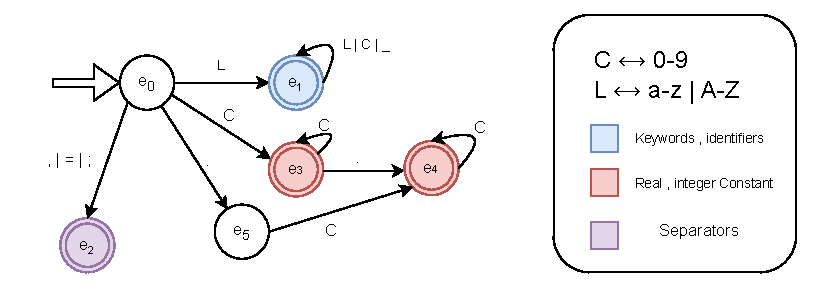
\includegraphics[height=0.3\textheight]{Exercices/EX4/ex4.drawio.pdf}
\end{center}


\begin{algorithm}
\caption{Algorithm Recognition}
\begin{algorithmic}[1]
\debut
\lire{Entity}   \com{1.95}{Reads token}
\State t\(_{c}\) \affect Entity[0]; \com{1.6}{Initialize with 1st character} 
\State E\(_{c}\) \affect e\(_0\); \com{2.53}{Intialize with initial state}
\State F \affect \{e\(_1\),e\(_2\),e\(_3\),e\(_4\)\}; \com{1.1}{List Of Final States}
\State cmpt \affect 0; \com{4}{Initialize counter of nb character}
\State keyword \affect \{\str{INT} , \str{REAL}\}; \com{0.6}{List of keywords}
\vspace{0.7em}
\While{( E\(_{c}\)\pase \vide\et t\(_c\) \pase \str{\#} )} \com{0.5}{Loop as long as there is no blockage and not all character of the token have been analyzed}
\vspace{0.25em}
\State E\(_c\) \affect M[E\(_c\),t\(_c\)]; \com{1}{Gets next state}
\State t\(_c\) \affect t\(_s\);\com{2.2}{Gets next character of the token}
\State cmpt \affect cmpt + 1; \com{0.4}{Increment Counter}
\vspace{0.25em}
\EndWhile

\vspace{0.7em}

\If{( E\(_c\)\pase \vide )} \com{1}{Check if there is a blockage}

\vspace{0.25em}
\pr{Error the lexical entity isn't regonised by the automaton because blockage happened}

\vspace{0.25em}
\ElsIf{( E\(_c\) \nin F )} \com{1}{Check if automaton reaches a final state}

\vspace{0.25em}
\pr{Error the lexical entity isn't regonised by the automaton because it didn't reach a final state}

\vspace{0.25em}
\Else  
\If{( E\(_c\) \y e\(_1\) )}  \com{1}{Check if identifier or keyword}
\If {( Entity  \dn keyword )} \com{1}{Check if keyword}
\State Codify the keyword and put it in the symbole table.

\vspace{0.15em}
\Else \com{1}{Token is identifier} 
\If{( cmpt \g 7 )} \com{1}{Check length of identifier}
\pr{Error the identifier exceeded the maximum character length}
\Else
\State Codify the identifier and put it in the symbole table.
\EndIf
\EndIf

\vspace{0.15em}
\ElsIf {( E\(_c\) \y e\(_3\) )} \com{1}{Check if integer constant}
\If{ (cmpt \g 5) } \com{1}{Check length of integer constant}
\pr{Error the integer constant exceeded the maximum character lenght}
\ElsIf {(\ev{Entity} \g 32768)} \com{1}{Check value of integer constant}
\pr{Error the integer constant exceeded the maximum possible value}
\Else
\State Codify the integer constant and put it in the symbole table.
\EndIf

\vspace{0.15em}
\ElsIf {( E\(_c\) \y e\(_4\) )} \com{1}{Check if float constant}
\If{ (cmpt \g 9) } \com{1}{Check length of float constant}
\pr{Error the float constant exceeded the maximum character lenght}
\Else
\State Codify the float constant and put it in the symbole table.
\EndIf

\vspace{0.15em}
\Else \com{1}{token is a separator}
\State Codify the seperator and put it in the symbole table.
\EndIf
\vspace{0.25em}

\vspace{0.25em}
\EndIf
\fin
\end{algorithmic}
\end{algorithm}

\null
\newpage

\begin{prettyBox}{Note}{red}
\begin{itemize}
    \item Identifiers and keywords share the same branch in the automaton to simplify its structure.  
          In the recognition algorithm, we will store the keywords in an array and compare them with the token.  
    \item In most compiler notations, formats like `.25` (meaning `0.25`) and `45.` (meaning `45.0`) are accepted.  
    \item Eval convert string into integer.
\end{itemize}
\end{prettyBox}


